%%%%%%%%%%%%%%%%%%%%%%%%%%%%%%%%%%%%%%%%%%%%%%%%%%%%%%%%%%%%%%%%%%%%%%%%%%%%%%%%
%                         FORMATO DE TESIS UMSNH                               %
%%%%%%%%%%%%%%%%%%%%%%%%%%%%%%%%%%%%%%%%%%%%%%%%%%%%%%%%%%%%%%%%%%%%%%%%%%%%%%%%
% based on Harish Bhanderi's PhD/MPhil template, then Uni Cambridge
% http://www-h.eng.cam.ac.uk/help/tpl/textprocessing/ThesisStyle/
% corrected and extended in 2007 by Jakob Suckale, then MPI-iCBG PhD programme
% and made available through OpenWetWare.org - the free biology wiki
% forked from https://github.com/Tepexic/Tesis-UNAM on July 2017
% modifications made by Arturo Lopez Pineda

%                     Under GNU License v3
% ADAPTADO PARA UMSNH:  @arturolp
% ADAPTADO PARA PUCP:  @liskoc
\documentclass[oneside,11pt]{Latex/Classes/thesisUMSNH}
%  PUEDEN INCLUIR EN ESTE ESPACIO LOS PAQUETES EXTRA, O BIEN, EN EL ARCHIVO "PhDthesisPSnPDF.cls" EN "./Latex/Classes/"
\usepackage{blindtext}  % Para insertar texto dummy, de ejemplo, pues.
%\usepackage[round, sort, numbers]{natbib}  % Personalizar la bibliografía
\usepackage{natbib}
%\usepackage{apacite}
\usepackage{minted} % Enbelleciminiento de código
% This file contains macros that can be called up from connected TeX files
% It helps to summarise repeated code, e.g. figure insertion (see below).

%%%%%%%%%%%%%%%%%%%%%%%%%%%%%%%%%%%%%%%%%%%%%%
%            Colores de la UNAM              %
%%%%%%%%%%%%%%%%%%%%%%%%%%%%%%%%%%%%%%%%%%%%%%
% Para UNAN: Azul Pantone 541  -->(0,63,119) RGB
% Para UMSNH: PANTONE Blue 072 C
\definecolor{Azul}{RGB}{51,51,153}

% Para UNAM: Oro Pantone 460  -->(234,221,150) RGB
% Para UMNSH: PANTONE 110 C
\definecolor{Oro}{RGB}{204,153,51}


%%%%%%%%%%%%%%%%%%%%%%%%%%%%%%%%%%%%%%%%%%%%%%
%            Comandos para líneas            %
%%%%%%%%%%%%%%%%%%%%%%%%%%%%%%%%%%%%%%%%%%%%%%
%Se define un comando \colorvrule para hacer líneas verticales de color con 3 argumentos: color, ancho, alto
\newcommand{\colorvrule}[3]{
\begingroup\color{#1}\vrule width#2 height#3
\endgroup}

%Se define un comando \colorhrule para hacer líneas horizontales de color con 2 argumentos: color, ancho
\newcommand{\colorhrule}[2]{
\begingroup\color{#1}\hrule height#2
\endgroup}

%%%%%%%%%%%%%%%%%%%%%%%%%%%%%%%%%%%%%%%%%%%%%%
%          Comando para derivadas            %
%%%%%%%%%%%%%%%%%%%%%%%%%%%%%%%%%%%%%%%%%%%%%%
\newcommand{\derivada}[3][]{\ensuremath{\dfrac{\mbox{d}^{#1}#2}{\mbox{d}#3^{#1}}}} 
%primer argumento(opcional): orden de la derivada
%segundo argumento: función a derivar
%tercer argumento: variable respecto a la que se deriva


%%%%%%%%%%%%%%%%%%%%%%%%%%%%%%%%%%%%%%%%%%%%%%
%       Comando para la exponencial          %
%%%%%%%%%%%%%%%%%%%%%%%%%%%%%%%%%%%%%%%%%%%%%%
\newcommand{\e}[1][]{\ensuremath{\mbox{e}^{#1}}}
%primer argumento(opcional): exponente de la exponencial




% insert a centered figure with caption and description
% parameters 1:filename, 2:title, 3:description and label
\newcommand{\figuremacro}[3]{
	\begin{figure}[htbp]
		\centering
		\includegraphics[width=1\textwidth]{#1}
		\caption[#2]{\textbf{#2} - #3}
		\label{condicion}
	\end{figure}
}

% insert a centered figure with caption and description AND WIDTH
% parameters 1:filename, 2:title, 3:description and label, 4: textwidth
% textwidth 1 means as text, 0.5 means half the width of the text
\newcommand{\figuremacroW}[4]{
	\begin{figure}[htbp]
		\centering
		\includegraphics[width=#4\textwidth]{#1}
		\caption[#2]{\textbf{#2} - #3}
		\label{#1}
	\end{figure}
}

% inserts a figure with wrapped around text; only suitable for NARROW figs
% o is for outside on a double paged document; others: l, r, i(inside)
% text and figure will each be half of the document width
% note: long captions often crash with adjacent content; take care
% in general: above 2 macro produce more reliable layout
\newcommand{\figuremacroN}[3]{
	\begin{wrapfigure}{o}{0.5\textwidth}
		\centering
		\includegraphics[width=0.48\textwidth]{#1}
		\caption[#2]{{\small\textbf{#2} - #3}}
		\label{#1}
	\end{wrapfigure}
}

% predefined commands by Harish
\newcommand{\PdfPsText}[2]{
  \ifpdf
     #1
  \else
     #2
  \fi
}

\newcommand{\IncludeGraphicsH}[3]{
  \PdfPsText{\includegraphics[height=#2]{#1}}{\includegraphics[bb = #3, height=#2]{#1}}
}

\newcommand{\IncludeGraphicsW}[3]{
  \PdfPsText{\includegraphics[width=#2]{#1}}{\includegraphics[bb = #3, width=#2]{#1}}
}

\newcommand{\InsertFig}[3]{
  \begin{figure}[!htbp]
    \begin{center}
      \leavevmode
      #1
      \caption{#2}
      \label{#3}
    \end{center}
  \end{figure}
}







%%% Local Variables:
%%% mode: latex
%%% TeX-master: "~/Documents/LaTeX/CUEDThesisPSnPDF/thesis"
%%% End:
           % Archivo con funciones útiles
\hypersetup{colorlinks=true, linkcolor=blue, citecolor=blue, filecolor=blue, urlcolor=blue, pdftitle=, pdfauthor=, pdfsubject=, pdfkeywords=}
\usepackage[pdftex]{graphicx}


%%%%%%%%%%%%%%%%%%%%%%%%%%%%%%%%%%%%%%%%%%%%%%%%%%%%%%%%%%%%%%%%%%%%%%%%
%                                   DATOS                                      %
%%%%%%%%%%%%%%%%%%%%%%%%%%%%%%%%%%%%%%%%%%%%%%%%%%%%%%%%%%%%%%%%%%%%%%%%%%
\title{Cálculo del viento en parque eólicos sobre terrenos complejos usando los métodos RANS y Lattice-Boltzman}
\author{Luis Koc} 
\facultad{ESCUELA DE POSGRADO}                 % Nombre de la facultad/escuela
\escudofacultad{Latex/Classes/Escudos/logo_pucp.jpeg} % Aquí ponen la ruta
%y nombre del escudo de su facultad, actualmente, la carpeta
%Latex/Classes/Escudos 

\degree{Maestría en Energía}   % Carrera
\director{Dr. Luis Chirinos}     % Director de tesis
\tutor{Dr. Luis Chirinos}      % Tutor de tesis, si aplica
\degreedate{2020}              % Año de la fecha del examen
\lugar{Lima, Perú}             % Lugar

%\portadafalse                 % Portada en NEGRO, descomentar y comentar la línea siguiente si se quiere utilizar
\portadatrue                   % Portada en COLOR

%% Opciones del posgrado (descomentar si las necesitan)
	\posgradotrue                                                    
	\programa{ESCUELA DE POSGRADO}
	\campo{MAESTRÍA EN ENERGÍA}
	%% En caso de que haya comité tutor
	%\comitetrue
	%\ctutoruno{Dr. Emmet}
	%\ctutordos{Dr. Doctor}
%% Datos del jurado                             
	%\presidente{Dr. 1}
	%\secretario{Dr. 2}
	%\vocal{Dr. 3}
	%\supuno{Dr. 4}
	%\supdos{Dr. 5}
	%\institucion{el Instituto de Ingeniería, UNAM}
\keywords{CFD,viento,eólico,parques eólicos,simulación,OpenFoam} % Palablas clave para los metadatos del PDF
\subject{Parques Eólicos,Mecánica de fluidos computacional}      % Tema para metadatos del PDF  
%%%%%%%%%%%%%%%%%%%%%%%%%%%%%%%%%%%%%%%%%%%%%%%%%%%%%
%                   PORTADA                         %
%%%%%%%%%%%%%%%%%%%%%%%%%%%%%%%%%%%%%%%%%%%%%%%%%%%%%
\begin{document}

\maketitle	% Se redefinió este comando en el archivo de la clase para generar automáticamente la portada a partir de los datos

%%%%%%%%%%%%%%%%%%%%%%%%%%%%%%%%%%%%%%%%%%%%%%%%%%%%%
%                  PRÓLOGO                          %
%%%%%%%%%%%%%%%%%%%%%%%%%%%%%%%%%%%%%%%%%%%%%%%%%%%%%
\frontmatter
\begin{dedication}
	
A Karina L., " porque la luna nunca brilla sin traerme tus sueños, y las estrellas nunca aparecen sin que yo sienta tus ojos brillantes" \cite{poe_annabel_2014} \\
\bigskip

\end{dedication}
       % Comentar línea si no se usa
%\chapter*{}
%\pagenumbering{Roman}

\begin{acknowledgements}

A mis hijos Joaquín y Karina, sin cuya amable ayuda, comprensión y tolerancia con mis tareas imposibles, este trabajo nunca hubiera sido realizado.\\


%\blindtext % Dummy text
\end{acknowledgements}




   % Comentar línea si no se usa 
% ******************************* Thesis Declaration ********************************

\begin{declaration}

Por la presente declaro que, excepto cuando se haga referencia específica al trabajo de otras personas, el contenido de esta tesis es original y no se ha presentado total o parcialmente para su consideración para cualquier otro título o grado en esta o alguna otra Universidad. Esta tesis es resultado de mi propio trabajo y no incluye nada que sea el resultado de algún trabajo realizado en colaboración, salvo que se indique específicamente en el texto.
% Author and date will be inserted automatically from thesis.tex


\end{declaration}
           % Comentar línea si no se usa

% Thesis Abstract -----------------------------------------------------


%\begin{abstractslong}    %uncommenting this line, gives a different abstract heading
\begin{abstracts}        %this creates the heading for the abstract page

El problema de calcular los perfiles de velocidad del viento sobre terrenos complejos ha recibido gran atención en los últimos años debido al incremento de la generación eléctrica con turbinas eólicas en, prácticamente, todos los países del mundo. La información obtenida mediante la solución numérica de las ecuaciones de Navier-Stokes puede agilizar el desarrollo de los proyectos eólicos permitiendo una mejor estimación del recurso energético que hace viable a este tipo de proyectos.
\\
\\
\hspace*{1em} Un balance entre esfuerzo computacional y precisión de los resultados es requerido; así las ecuaciones de promedios de Reynold (RANS) y la caracterización de la  turbulencia mediante modelos de transporte de la energía cinética turbulenta y el ratio de disipación de esta energía (modelo $\kappa$-$\epsilon$ ) en estado estable han sido usados en el presente trabajo. Así mismo, la interacción entre el flujo turbulento del aire, los terrenos con topografía compleja y la capa límite atmosférica son analizadas, adicionalmente en estado dinámico utilizando el método de lattice-Boltzman (LBM).
\\
\\
\hspace*{1em}Se presenta una metodología para calcular la velocidad de viento, intensidad de turbulencia y otras magnitudes relevantes en las áreas extensas sobre la que se construyen parques eólicos. El calculo incluye valores a diferentes altitudes; así como, la interacción con las turbinas eólicas de modos que se estiman las pérdidas por estelas. Se utilizan los métodos RANS $\kappa$-$\epsilon$ (usando el código OpenFoam) y Lattice-Boltzman (usando el código OpenLB). Los resultados son validados mediante la resolución de problemas canónicos y comparaciones con valores medidos en el campo obteniendo resultados consistentes.


%\blindtext

\end{abstracts}
%\end{abstractlongs}


% ----------------------------------------------------------------------                   % Comentar línea si no se usa

%%%%%%%%%%%%%%%%%%%%%%%%%%%%%%%%%%%%%%%%%%%%%%%%%%%%%
%                   ÍNDICES                         %
%%%%%%%%%%%%%%%%%%%%%%%%%%%%%%%%%%%%%%%%%%%%%%%%%%%%%
%Esta sección genera el índice
\setcounter{secnumdepth}{3} % organisational level that receives a numbers
\setcounter{tocdepth}{3}    % print table of contents for level 3
\tableofcontents            % Genera el índice 
%: ----------------------- list of figures/tables ------------------------
\listoffigures              % Genera el ínidce de figuras, comentar línea si no se usa
\listoftables               % Genera índice de tablas, comentar línea si no se usa


%%%%%%%%%%%%%%%%%%%%%%%%%%%%%%%%%%%%%%%%%%%%%%%%%%%%%
%                   CONTENIDO                       %
%%%%%%%%%%%%%%%%%%%%%%%%%%%%%%%%%%%%%%%%%%%%%%%%%%%%%
% the main text starts here with the introduction, 1st chapter,...
\mainmatter
\def\baselinestretch{1.5}                   % Interlineado de 1.5

% this file is called up by thesis.tex
% content in this file will be fed into the main document
%----------------------- introduction file header -----------------------
%%%%%%%%%%%%%%%%%%%%%%%%%%%%%%%%%%%%%%%%%%%%%%%%%%%%%%%%%%%%%%%%%%%%%%%%%
%  Capítulo 1: Introducción- DEFINIR OBJETIVOS DE LA TESIS              %
%%%%%%%%%%%%%%%%%%%%%%%%%%%%%%%%%%%%%%%%%%%%%%%%%%%%%%%%%%%%%%%%%%%%%%%%%

\chapter{Introducción}

%: ----------------------- HELP: latex document organisation
% the commands below help you to subdivide and organise your thesis
%    \chapter{}       = level 1, top level
%    \section{}       = level 2
%    \subsection{}    = level 3
%    \subsubsection{} = level 4
%%%%%%%%%%%%%%%%%%%%%%%%%%%%%%%%%%%%%%%%%%%%%%%%%%%%%%%%%%%%%%%%%%%%%%%%%
%                           Presentación                                %
%%%%%%%%%%%%%%%%%%%%%%%%%%%%%%%%%%%%%%%%%%%%%%%%%%%%%%%%%%%%%%%%%%%%%%%%%

\section{Presentación} % section headings are printed smaller than chapter names

Las emisiones de carbono, lejos de reducirse, han ido en aumento en los últimos años. Entre el 2002 y 2011  crecieron con ua ratio anual de $3.2\ \%$ en promedio \citep[p.~50]{stocker_climate_2013}. Para el año 2017, el ratio de crecimiento ha sido estimado en $1.8\ \%$ \citep[p.~2]{peters_towards_2017}. Una gran proporción de estas emisiones provienen de la industria de la energía eléctrica, de tal modo que existe la necesidad de llevar a cabo una profunda descarbonización que permita atenuar los efectos del calentamiento global y el cambio climático. Las políticas de descarbonización  implican, entre otras cosas, un incremento de la generación de electricidad con recursos energéticos renovables que reemplacen  las actuales fuentes que utilizan combustibles fósiles \citep[p.~3]{duan_modeling_2020}.

Desde el año 2010, el estado peruano viene impulsando la construcción de centrales de generación renovables [ citar Política energética nacional]. De ese modo existen actualmente 300 megavatios de generación eléctrica que utilizan fuentes renovables principalmente Eólicas, solar fotovoltaica y biomasa que cubren el 3.8\% de la demanda de energía eléctrica del país, como está reportado en \citep{coes_memoria_2016}.

En la última década, los proyectos de generación renovables, se han desarrollado no sin problemas en nuestro País. Estos proyectos, en el corto plazo están limitados a los sitios con recurso de alta calidad (el sur para la generación solar fotovoltaica y la costa centro y norte para la generación eólica). De otro lado, el desarrollo de estos proyectos puede llevar a conflictos, como ha ocurrido en países con mayor penetración de energías renovables. En particular, los proyectos eólicos han tenido oposición debido a la intrusión visual, contaminación por ruido, daño a las aves, entre otras razones \citep[p.~282]{moriarty_energy_2018}.


%como se puede apreciar en la figura \ref{fig:sankeyperu2013}
%
%\begin{figure} [h!]
%\centering
%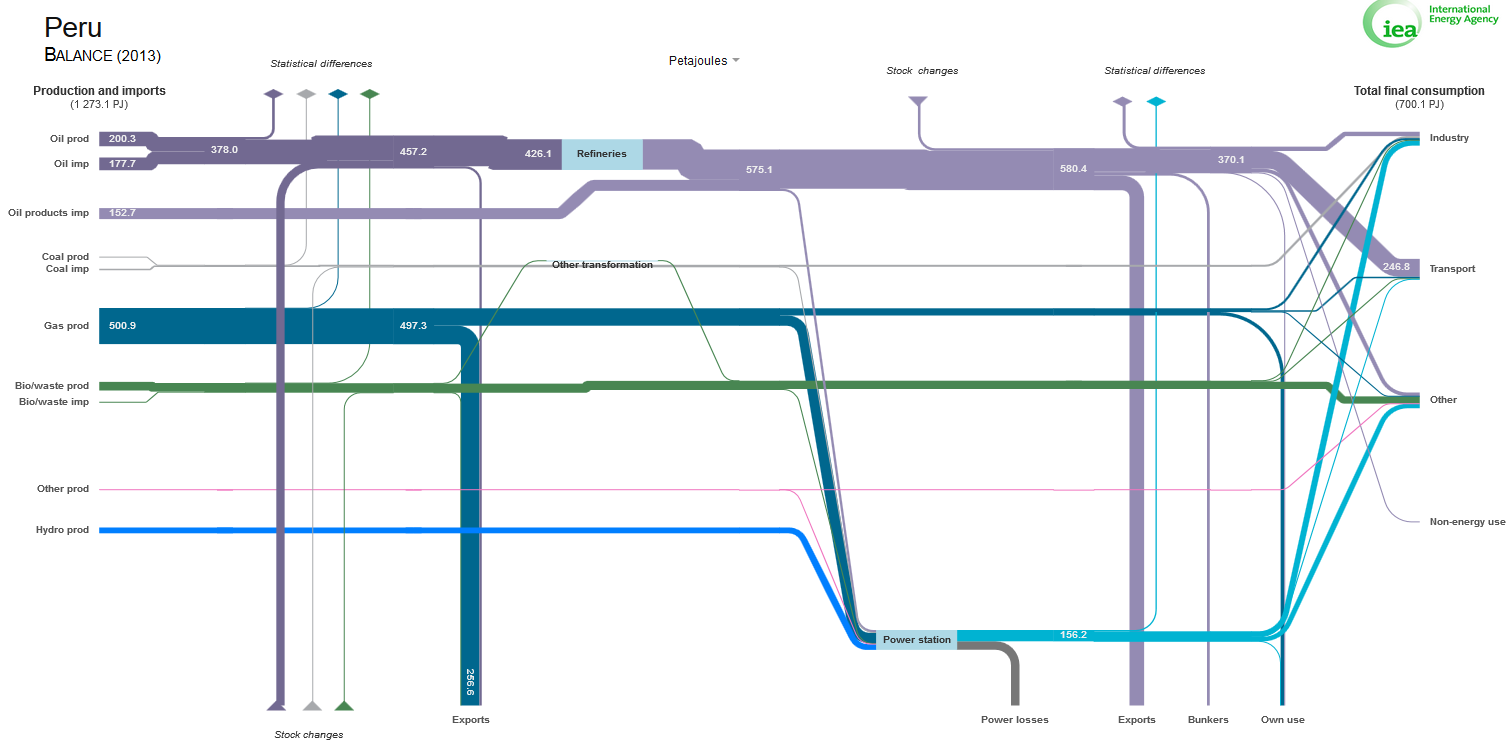
\includegraphics[width=0.80\linewidth]{imagenes/sankey_peru_2013}
%\caption[Diagrama de Sankey - Perú 2013]{Diagrama de Sankey - Perú 2013 (Fuente:\citep{iea_iea_2016} }
%\label{fig:sankeyperu2013}
%\end{figure}

Actualmente la generación de energía eléctrica eléctrica está "gasificada", considerando los bajos precios de gas provenientes  del lote 88. La participación de la energía eléctrica termoeléctrica (prácticamente producida toda con gas natural) tiene un porcentaje de participación similar a la energía hidroeléctrica y con una tendencia creciente [cita requerida de la memoria anual COES]. 
La actual construcción del gaseoducto al Sur y las nuevas plantas denominadas “Nodo energético” en Ilo y Mollendo, profundizarán e incrementarán el predominio del gas natural en la matriz energética nacional. Se espera así mismo incrementos en la participación de energías renovables (eólicas, solar y mini hidroeléctricas) pero  la participación de éstas  será minoritaria en el corto y mediano plazo \citep{coes_memoria_2016}.



%%%%%%%%%%%%%%%%%%%%%%%%%%%%%%%%%%%%%%%%%%%%%%%%%%%%%%%%%%%%%%%%%%%%%%%%%
%                           Objetivo                                    %
%%%%%%%%%%%%%%%%%%%%%%%%%%%%%%%%%%%%%%%%%%%%%%%%%%%%%%%%%%%%%%%%%%%%%%%%%

\section{Objetivo}

Este trabajo tiene por objetivo ...



%(Generales y específicos.)
\subsection{Objetivo General}

Cuantificar la energía producida por parques eólicos usando técnicas de Mecánica de Fluidos Computacional (CFD) y Modelos de Mesoescala de Predicción Numérica  Meteorológicos (NWP) utilizando el software OpenFOAM.

\subsection{Objetivos Específicos}

\begin{itemize}

\item Entender los fenómenos de mecánicas de fluidos involucrados en el funcionamiento de los parques eólicos
\item Modelar las características topográficas de la localización del Parque Eólico
\item Definir el tipo y modelo de turbinas eólicas que se analizarán.
\item Definir el arreglo general y ubicación de las turbinas eólicas
\item Definir el modelo simplificado  de intercambio de energía entre el flujo de viento y las turbinas eólicas. 
\item Definir las condiciones de frontera del volumen de control bajo estudio a partir de modelos numéricos climatológicos de meso-escala.
\item Elaboración de malla apropiada para los cálculos en el software OpenFOAM.
\item Determinar el tipo de flujo para usar el módulo apropiado del software OpenFOAM
\item Implementar el modelo utilizando el sofware OpenFOAM
\item Cuantificar la producción de energía para diferentes condiciones de operación y diferentes condiciones meteorológicas utilizando la similación numérica en OpenFOAM.
\item Comparar los resultados obtenidos con mediciones de campo existentes.
\item Evaluar los resultados obtenidos.
\end{itemize}

%%%%%%%%%%%%%%%%%%%%%%%%%%%%%%%%%%%%%%%%%%%%%%%%%%%%%%%%%%%%%%%%%%%%%%%%%
%                           Motivación y estado del arte                %
%%%%%%%%%%%%%%%%%%%%%%%%%%%%%%%%%%%%%%%%%%%%%%%%%%%%%%%%%%%%%%%%%%%%%%%%%
\section{Motivación}

El problema de calcular el viento sobre terrenos complejos ha recibido gran atención en los últimos años debido al incremento de la generación eléctrica con turbinas eólicas en diversas partes del mundo. La simulación numérica mediante la discretización de las ecuaciones de Navier-Stokes agiliza el desarrollo de los proyectos eólicos mediante una mejor estimación del recurso energético que hace viable a este tipo de proyectos.
\\
\\\subsection{Parque Eólicos}
En el caso de los Parque Eólicos, la producción de energía eléctrica depende de las características técnicas de los aerogeneradores las cuales son informadas por los fabricantes y por la disponibilidad del recurso eólico, que requiere de mediciones de largo plazo, \footnote{En las referencias  \citep{wbank_guidelines_2014}, \citep{sanz_state---art_2010} y \citep{bailey_wind_1997} se recomiendan tener un año de mediciones como mínimo aunque tres o cinco años son preferidos}. Estas mediciones se toman con un período de 10 minutos que incluyen velocidad y dirección del viento a diversas alturas entre 60 m y 100 m utilizando  sensores instalados en torres de medición instalada en el campo. 

Las mediciones de largo plazo tiene como objetivo de capturar las variaciones de largo plazo y reducir la incertidumbre de la medición. Dependiendo de la extensión del área y la complejidad de la topografía en la que estará emplazado el parque eólico pueden requerirse varias torres de medición que permitan cuantificar el recurso eólico en una localización específica, considerando que las torres registran medidas de velocidad y dirección del viento en un solo punto geográfico.

\subsection{Modelos Numéricos y Computacionales}

En la referencia \citep{wbank_guidelines_2014} se recomienda la realización de análisis basados en Mecánica de Fluidos Computacinal  (CFD) cuando otras técnicas simplificadas no permitan obtener resultados satisfactorios de extrapolación de las mediciones, esto suele ocurrir en casos con terreno complejos e inestabilidades que carecen de homogeneiodad del flujo como es asumido por las técnicas de medición de campo \citep{sanz_state---art_2010}.

Con la finalidad de mejorar la cuantificación de la energía producida por los parques eólicos se han propuestos diversas metodologías que combinan la Técnicas de Mecánica de Fluidos Computacional (CFD) y Modelos de Mesoescala de Predicción Numérica  Meteorológicos (NWP). 

Los modelos NWP del nivel de mesoescala permiten establecer condiciones de frontera de temperatura, presión y velocidad de viento para realizar cálculos locales en áreas algunas decenas de kilómetros cuadrados. 

Los modelos de CFD deben permitir retener la no linealidad de las ecuaciones de Navier Stokes tomando en cuenta el balance de momento los fenómenos de turbulencia adaptados a los flujos atmosféricos \citep{sanz_state---art_2010}. 


\subsection{Modelos CFD y NWP utilizados en la cuantificacion de Recursos de Parques Eólicos}

Las Mecánica  de Fluidos Computacional (CFD) (acotar a un tipo de técnica de CFD) y los Modelos Numéricos de Predicción Meteorológica requieren conocimientos extensos de Métodos Numéricos, lenguajes de programación, Mecánica de Fluidos, entre otros que no se estudian en los Planes de Estudio de Pre-grado de ingeniería, por lo cual constituye un tema apropiado para ser propuesto como tesis de maestría.

En \citep{beaucage_more_????} se indica que el modelo ampliamente aceptado de predecir la variación espacial de la velocidad promedio del viento es un modelo linealizado de flujo de viento\footnote{Los softwares para producir mapas de viento utilizan ampliamente este tipo de técnicas de bajo costo computacional}, considerando a las técnicas basadas en CFD como la siguiente generación para aplicaciones de energía. 

Los modelos numéricos acoplados con motores de calculo meteorológicos y de predicción del tiempo permiten una mayor sofisticación del cálculo a la vez que incrementan los requerimientos computaciones de las simulaciones, aunque este incremento computacional puede ser soportado por los computadoras disponibles hoy en día, como se observa en \citep*{zajaczkowski_preliminary_2011}. 

Estos modelos sofisticados han sido investigados tanto por instituciones como NREL, Universidad de Chalmers y otras así como soluciones comerciales propuestas por compañías consultoras como AWS. 

NREL (National Renewable Energy Laboratory) desarrolló un software prototípico "SOWFA" (Simulator fOr Wind Farm Application) que utiliza el software OpenFOAM acoplado con un modelo LES (Large Eddy Simulation) o RANS (Reynolds Average Navier-Stokes) \citep{stull_introduction_2012}. 

AWS ha investigado el desempeño de cuatro modelos numéricos (Jackson-Hunt, RANS CFD, NWP-Mass Consistent y NWP-LES) obteniendo desempeños que varían grandemente de sitio a sitio y considerando promisorio el modelo NWP-LES \cite{brower_evaluation_2013}.

\cite{bengtsson_turbulence_????} ha comparado modelos lineas, modelos CFD y modelos NWT, obteniendo mejores resultados con el método CFD.

\subsection{El software OpenFOAM}

OpenFOAM (acrónimo de ``Open source Field Operation And Manipulation") es una herramienta de cálculo programada en el lenguaje C++ orientada al desarrollo de motores de cálculo especializados, utilidades de pre y pos-procesamiento para la solución de problemas de mecánica continua.

OpenFOAM posee librerías  para la resolución de problemas de Mecánica de Fluidos Computacional (CFD). El código es libre y fuente abierta por lo que puede ser analizado y modificado en sus detalles \citep*{wikipedia_openfoam_2016}.




%%%%%%%%%%%%%%%%%%%%%%%%%%%%%%%%%%%%%%%%%%%%%%%%%%%%%%%%%%%%%%%%%%%%%%%%%
%                   Planteamiento del problema                          %
%%%%%%%%%%%%%%%%%%%%%%%%%%%%%%%%%%%%%%%%%%%%%%%%%%%%%%%%%%%%%%%%%%%%%%%%%

\section{Planteamiento del problema}


La cuantificación de la energía requiere mediciones de largo plazo de la velocidad y dirección del viento que permitan cuantificar el recurso eólico disponible en el emplazamiento del parque eólico. Las mediciones de campo se llevan a cabo mediante anemómetros y veletas localizados a diferentes alturas en las torres de medición. Con la información obtenida de estos sensores se estima la energía disponible en una localización específica a lo largo de la vida útil del parque eólico. 

Dependiendo de la extensión del emplazamiento y de la complejidad de la topografía del terreno pueden requerirse varias torres de medición para obtener una cuantificación confiable del recurso eólico. 

Las metodologías basadas únicamente en mediciones de campo tienen la desventaja de tomar en cuenta de manera muy pobre el impacto de la topografía y las variaciones locales del viento. Esto es así debido a la naturaleza discreta de la medición (una torre registra datos de un solo punto), a las dificultades prácticas de instalar una gran cantidad de torres de medición y a los errores inherentes a la extrapolación de la data medida en una área geográfica extensa.

La predicción de la energía producida por futuros Parques Eólicos puede mejorarse usando modelos de Mecánica de Fluidos Computacional (CFD) que retengan las características no lineales de las ecuaciones de Navier-Stokes como el balance de momento y los fenómenos turbulentos. Este modelo toma como condiciones de frontera los resultados de Modelos de Mesoescala de Predicción Numérica  Meteorológicos (NWP) correspondientes en un lugar y sitio específico donde está o estará localizado el Parque Eólico. 


%%%%%%%%%%%%%%%%%%%%%%%%%%%%%%%%%%%%%%%%%%%%%%%%%%%%%%%%%%%%%%%%%%%%%%%%%
%                           Metodología                                 %
%%%%%%%%%%%%%%%%%%%%%%%%%%%%%%%%%%%%%%%%%%%%%%%%%%%%%%%%%%%%%%%%%%%%%%%%%
\section{Metodología}

Se tiene un objetivo principal, y para llegar a \'el %otra forma de poenr acentos


así las ecuaciones de promedios de Reynold (RANS) y la caracterización de la  turbulencia mediante modelos de transporte de la energía cinética turbulenta y el ratio de disipación de esta energía (modelo $\kappa$-$\epsilon$ ) en estado estable han sido usados en el presente trabajo. Así mismo, la interacción entre el flujo turbulento del aire, los terrenos con topografía compleja y la capa límite atmosférica son analizadas, adicionalmente en estado dinámico utilizando el método de lattice-Boltzman (LBM).
\\
\\
\hspace*{1em}Se presenta una metodología para calcular la velocidad de viento, intensidad de turbulencia y otras magnitudes relevantes en las áreas extensas sobre la que se construyen parques eólicos. El calculo incluye valores a diferentes altitudes; así como, la interacción con las turbinas eólicas de modos que incluyen las pérdidas por estelas. Se utilizan los métodos RANS $\kappa$-$\epsilon$ (usando el código OpenFoam) y Lattice-Boltzman (usando el código OpenLB). Los resultados son validados mediante la resolución de problemas canónicos y comparaciones con valores medidos en el campo obteniendo resultados consistentes.

%Planteamiento de las ecuaciones:	5
%Discretización de las ecuaciones.	7
%Elaboración del mallado decalado (staggered grid).	8

\begin{itemize}
	\item Se propone una implementación de la cuantificación del Recurso Eólico de un parque  utilizando un enfoque físico (enfoque determinista) en oposición a un enfoque estadístico \citep*{wang_review_2011}.

Este método físico estará basado predicción de las condiciones de la baja atmósfera o predicción meteorológica  (NWP) usando los datos como temperatura, presión, rugosidad de la superficie y obtaculos.

\item En general, la velocidad de viento es obtenida de los Sistemas que ofrecen información sobre condiciones meteorológicas \citep*{wang_review_2011}. 

Pará el Perú esta información están disponible previsiones numéricas dos veces al día con el modelo regional Eta para los dominios: Perú (22 Km) y Sudamérica (32 Km). Las condiciones iniciales y de frontera son obtenidas del modelo Global Forecast System (GFS) \citep{senamhi_servicio_????}. 

\item La información topográfica es convertida a un formato utilizable en OpenFOAM desde data obtenida y procesadas en sistemas de información geográfica como GRASS o QGIS, como se describe en \citep{hardin_how_2013}.

\item Los modelos son resueltos en OpenFOAM y los resultados son analizados y evaluados.
\end{itemize}

En la figura \ref{fig:metodo} se observa la etapas que se seguirán para realizar los cálculos propuestos. ESte muestra un ejemplo tomado de \citep{stull_introduction_2012} en el cual requirió un tiempo de procesamiento de 21 horas para 750 segundos de simulación corriendo en un arreglo de 64 procesadores.

\begin{figure}[h!]
\centering
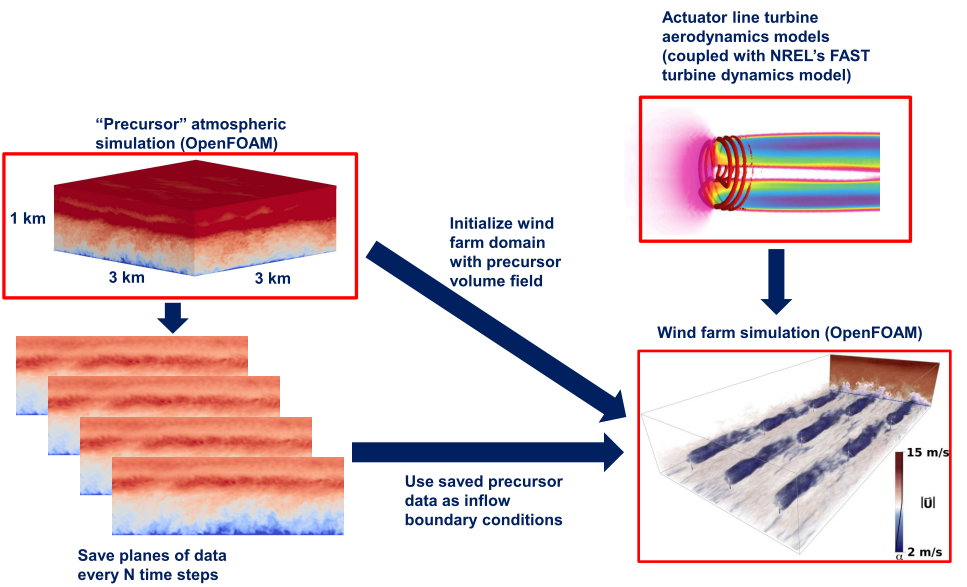
\includegraphics[width=0.8\linewidth]{imagenes/metodo}
\caption[Metodo de Cálculo]{Método de Cálculo (Fuente: \citep{stull_introduction_2012})}{}
\label{fig:metodo}
\end{figure}



%%%%%%%%%%%%%%%%%%%%%%%%%%%%%%%%%%%%%%%%%%%%%%%%%%%%%%%%%%%%%%%%%%%%%%%%%
%                         Contribuciones                                %
%%%%%%%%%%%%%%%%%%%%%%%%%%%%%%%%%%%%%%%%%%%%%%%%%%%%%%%%%%%%%%%%%%%%%%%%%

\section{Contribuciones}

La principal contribución de este trabajo es 
\blindtext
%%%%%%%%%%%%%%%%%%%%%%%%%%%%%%%%%%%%%%%%%%%%%%%%%%%%%%%%%%%%%%%%%%%%%%%%%
%                           Estructura de la tesis                      %
%%%%%%%%%%%%%%%%%%%%%%%%%%%%%%%%%%%%%%%%%%%%%%%%%%%%%%%%%%%%%%%%%%%%%%%%%

\section{Estructura de la tesis}

Este trabajo está dividido en XX capítulos. Al principio se encuentra 
\\\\
Finalmente se encuentra la parte de             % ~10 páginas - Explicar el propósito de la tesis

%%%%%%%%%%%%%%%%%%%%%%%%%%%%%%%%%%%%%%%%%%%%%%%%%%%%%%%%%%%%%%%%%%%%%%%%%
%           Capítulo 2: MARCO TEÓRICO - REVISIÓN DE LITERATURA
%%%%%%%%%%%%%%%%%%%%%%%%%%%%%%%%%%%%%%%%%%%%%%%%%%%%%%%%%%%%%%%%%%%%%%%%%

\chapter{Marco teórico}
En este capítulo, normalmete se ponen todas las ecuaciones que se van a usar en la tesis, así ya nomás se hace rferencia a la ecuación tal o "como se vió en el capítulo 2", y esas cosas.
%inserción de codigo de Matlab
%Es conveniente sangrarlo (los de proteco dicen "indentarlo") para que no se encime con los números  de las líneas a la izquierda
\begin{lstlisting}[frame=single]
    % Declaracion de las variables simbolicas
    syms u z1 z2 z3 z4 J m M g l 
    % Matrices involucradas
    E = [J+m*l*l m*l*cos(z1);m*l*cos(z1) M+m] 
    F = [m*g*l*sin(z1);u+m*l*(z3*z3)*sin(z1)] 
    % Despeje
    V = E\F
\end{lstlisting}

\blindtext           % ~20 páginas - Poner un contexto a la tesis, hacer referencia a trabajos actuales en el tema

%%%%%%%%%%%%%%%%%%%%%%%%%%%%%%%%%%%%%%%%%%%%%%%%%%%%%%%%%%%%%%%%%%%%%%%%%
%           Capítulo 3: NOMBRE                   %
%%%%%%%%%%%%%%%%%%%%%%%%%%%%%%%%%%%%%%%%%%%%%%%%%%%%%%%%%%%%%%%%%%%%%%%%%

\chapter{Diseño del experimento}
En este capítulo, se presenta la introducción al desarrollo de la tesis, ya sea el modelo matemático o las bases del proyecto, etc.
Ejemplo de cita  [\citet{latex}]
Ejemplo de cita [\citeauthor{RR73}]
 % The \cite command functions as follows:
 %   \citet{key} ==>>                Jones et al. (1990)
 %   \citet*{key} ==>>               Jones, Baker, and Smith (1990)
 %   \citep{key} ==>>                (Jones et al., 1990)
 %   \citep*{key} ==>>               (Jones, Baker, and Smith, 1990)
 %   \citep[chap. 2]{key} ==>>       (Jones et al., 1990, chap. 2)
 %   \citep[e.g.][]{key} ==>>        (e.g. Jones et al., 1990)
 %   \citep[e.g.][p. 32]{key} ==>>   (e.g. Jones et al., p. 32)
 %   \citeauthor{key} ==>>           Jones et al.
 %   \citeauthor*{key} ==>>          Jones, Baker, and Smith
 %   \citeyear{key} ==>>             1990





%%%%%%%%%%%%%%%%%%%%%%%%%%%%%%%%%%%%%%%%%%%%%%%%%%%%%%%%%%%%%%%%%%%%%%%%%
%                          Descripción de la planta                     %
%%%%%%%%%%%%%%%%%%%%%%%%%%%%%%%%%%%%%%%%%%%%%%%%%%%%%%%%%%%%%%%%%%%%%%%%%
\section{Sección}
El sistema blah, blah. Ejemplo de cita \citep{texbook}
La figura (\ref{planta})                     %hace referencia a la imagen "planta" el número se inserta automáticamente
 ilustra los componentes de la planta.

\begin{figure}
  \centering
    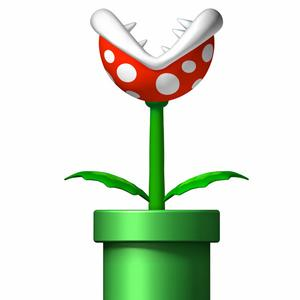
\includegraphics[scale=0.5]{Capitulo3/figs/planta.jpg}      %Ruta completa de la imagen, porque se compila desde el archivo tesis.tex
  \caption{Descripción de la planta}            %Pie de imagen
  \label{planta}                            %nombre de referencia
\end{figure}




%%%%%%%%%%%%%%%%%%%%%%%%%%%%%%%%%%%%%%%%%%%%%%%%%%%%%%%%%%%%%%%%%%%%%%%%%
%                          Modelado                                     %
%%%%%%%%%%%%%%%%%%%%%%%%%%%%%%%%%%%%%%%%%%%%%%%%%%%%%%%%%%%%%%%%%%%%%%%%%
\section{\textcolor{Azul}{Sección en color azul}}
\subsection{Subsección}
Antes de comenzar, se definen  en la tabla ~\ref{tab:tabla} los parámetros y variables utilizadas

%%%%%%%%Tabla Nombres de parámetros
\begin{table}[ht]                             %Inicia el entorno table debajo del texto
\centering\                                     %   centra la tabla
\begin{tabular}{||c | c ||}                     %inicia entorno tabular con doble línea en las orillas, 2 columnas con el contenido centrado (c)
\hline                                          %inserta línea horizontal
\hline
Nombre Parámetro/Variable & Símbolo\\
\hline
\hline
Masa del péndulo & $m$ \\
\hline
Masa del carro & $M$\\
\hline
Distancia del eje de giro al centro de masa & $l$ \\
\hline
Aceleración gravitatoria & $g$ \\
\hline
Momento de inercia péndulo respecto del eje de giro& $J$ \\
\hline
Ángulo del péndulo respecto del eje vertical & $\theta$\\
\hline
Velocidad angular del péndulo & $\dot{\theta}$, $\omega$\\
\hline
Distancia del carro respecto al centro del riel & x\\
\hline
Velocidad del carro & $\dot{x}$, $v$\\
\hline
\hline
\end{tabular}
\caption[Parámetros dinámicos del carro-péndulo]{\textbf{Parámetros dinámicos del carro-péndulo} - Estos son los valores de parámetros utilizados en el diseño y las simulaciones, corresponden a los valores reales.}
\label{tab:tabla}                              %etiqueta para referencia
\end{table}

\blindtext


%%%%%%%%%%%%%%%%%%%%%%%%%%%%%%%%%%%%%%%%%%%%%%%%%%%%%%%%%%%%%%%%%%%%%%%%%
%                          Subsección
%%%%%%%%%%%%%%%%%%%%%%%%%%%%%%%%%%%%%%%%%%%%%%%%%%%%%%%%%%%%%%%%%%%%%%%%%

\subsection{Otra subsección}

\Blindtext      % ~20 páginas - Explicar el problema en específico que se va a resolver, la metodología y experimentos/métodos utilizados
\chapter{Análisis de Resultados}
\section{Resultados}
\Blindtext   % ~20 páginas - Presentar los resultados tal cual son, y analizarlos.
\chapter{Conclusiones}
\blindtext            % ~5 páginas - Resumir lo que se hizo y lo que no y comentar trabajos futuros sobre el tema

%%%%%%%%%%%%%%%%%%%%%%%%%%%%%%%%%%%%%%%%%%%%%%%%%%%%%
%                   APÉNDICES                       %
%%%%%%%%%%%%%%%%%%%%%%%%%%%%%%%%%%%%%%%%%%%%%%%%%%%%%
\appendix
% this file is called up by thesis.tex
% content in this file will be fed into the main document
\chapter{Código/Manuales/Publicaciones}
% top level followed by section, subsection

\section{Apéndice}

Apéndice
               % Colocar los circuitos, manuales, código fuente, pruebas de teoremas, etc.

%%%%%%%%%%%%%%%%%%%%%%%%%%%%%%%%%%%%%%%%%%%%%%%%%%%%%
%                   REFERENCIAS                     %
%%%%%%%%%%%%%%%%%%%%%%%%%%%%%%%%%%%%%%%%%%%%%%%%%%%%%
% existen varios estilos de bilbiografía, pueden cambiarlos a placer
\bibliographystyle{apalike} % otros estilos pueden ser abbrv, acm, alpha, apalike, ieeetr, plain, siam, unsrt

%El formato trae otros estilos, o pueden agregar uno que les guste:
%\bibliographystyle{Latex/Classes/PhDbiblio-case} % title forced lower case
%\bibliographystyle{Latex/Classes/PhDbiblio-bold} % title as in bibtex but bold
%\bibliographystyle{Latex/Classes/PhDbiblio-url} % bold + www link if provided
%\bibliographystyle{Latex/Classes/jmb} % calls style file jmb.bst

\bibliography{Bibliografia/referencias}             % Archivo .bib


\end{document}
